\subsection{Deployment View}
\label{sec:deployment}

\begin{figure}[htb]
	\centering
	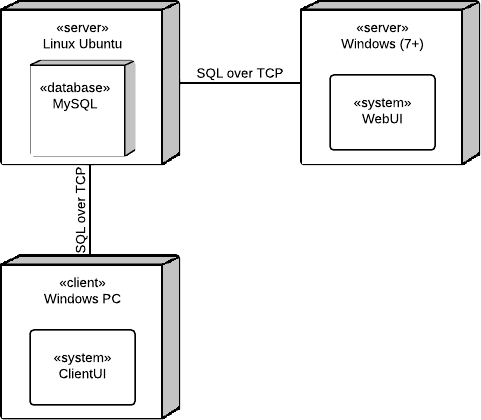
\includegraphics[width=0.7\textwidth]{Software_architecture/graphics/deployment-diag.png}
	\caption{Deployment Diagram of the application, showing its distribution.}
	\label{fig:deployment-diag}
\end{figure}

SliceOfPie has three different parts deployed: The database server, the web server and the local
desktop client.

{\bf The database server} has a Linux-based OS and hosts a remotely-accessible MySQL database
that is the central point of the application's network, holding the current online state. Having
a single database server ensures a consistent state across the platforms accessing the service.
It is, however, also a single point of failure. In a production environment this could be mitigated
by setting up a second server as a backup.

There are some security concerns with regards to having a remotely-accessible MySQL database that are
discussed in \ref{sec:mysqlvswebservice}.

{\bf The web-server} is a Windows server hosting a WebUI client. This client is accessible from all
locations that have access to the host. This means that a Web server may be set up anywhere to provide
a public interface for a great amount of users. Having the data separated from the web interface allows
for several such hosts to be running with the same consistent state. As handling requests, user-sessions,
and HTML transfers are often a bottleneck, simply sending users to different servers can be an advantage if the system receives a great
amount of traffic.

{\bf The desktop client} is a single client, which accesses the data-server directly. It has the advantage
of allowing users to work offline, without a connection to the internet, and synchronize with the global
state of the database server when they regain internet connection. Without synchronization, it also works
as a simple text-editor. It has the disadvantage of not being guaranteed up-to-date (like the Web UI is).